% Copyright 2017-2019 Remi Lehe
%
% This file is part of WarpX.
%
% License: BSD-3-Clause-LBNL


\usepackage{bm}
\usepackage{amsmath}
\usepackage{amssymb}
\usepackage{graphicx}
\usepackage{url}
\usepackage{hyperref}

\usepackage[displaymath]{lineno}\usepackage{bm}% bold math

\newcommand{\fe}{\mathbf{\tilde{E}}}
\newcommand{\fb}{\mathbf{\tilde{B}}}
\newcommand{\fj}{\mathbf{\tilde{J}}}
\newcommand{\ff}{\tilde{F}}
\newcommand{\fg}{\tilde{G}}
\newcommand{\fk}{\mathbf{k}}
\newcommand{\fkhat}{\mathbf{\hat{k}}}

% Definitions from Remi's paper on Galilean math
\newcommand{\Km}{\vec{K}_{\vec{m}}}
\newcommand{\km}{\vec{k}_{\vec{m}}}
\renewcommand{\vec}[1]{\boldsymbol{#1}}
\newcommand{\vgal}{\vec{v}_{gal}}
\newcommand{\nab}{\vec{\nabla'}}
\newcommand{\Dt}[1]{ \frac{\partial #1}{\partial t}}
\newcommand{\mc}[1]{\hat{\mathcal{#1}}}
\newcommand{\xj}{\vec{x}'_{\vec{j}}}
\newcommand{\Xll}{\vec{X}_{\vec{\ell}}}
\newcommand{\Integ}[1]{\int_{-\infty}^{\infty} \!\!\!\!\!\!
  \mathrm{d}#1}
\newcommand{\RInteg}[1]{\int_{0}^{\infty} \!\! \frac{#1\mathrm{d}#1}{(2\pi)^2}}

% Definitions from Remi's Thesis
\newcommand{\h}{\mathcal{H}}
\newcommand{\hf}{\frac{1}{2}}
\newcommand{\um}{$\mu$m}
\newcommand{\Um}{\mu \mathrm{m}}
\newcommand{\aal}{\langle \vec{a}_l^2 \rangle}
\newcommand{\etad}{ \eta_d }
\newcommand{\etae}{ \eta_\epsilon }
\newcommand{\etag}{ \eta_\gamma }
\newcommand{\tlambda}{ \tilde{\lambda} }
%\newcommand\comment[1]{\textcolor{red}{\textbf{#1}}}
\newcommand{\gsim}{\mathrel{\hbox{\rlap{\lower.55ex
\hbox{$\sim$}} \kern-.3em \raise.4ex \hbox{$>$}}}}
\newcommand{\lsim}{\mathrel{\hbox{\rlap{\lower.55ex
\hbox{$\sim$}} \kern-.3em \raise.4ex \hbox{$<$}}}}
\newcommand{\kfoc}{k_\mathrm{foc}}
\newcommand{\bkfoc}{\bar{k}_\mathrm{foc}}
\newcommand{\xil}{\xi_{\mathrm{laser}}}

\newcommand{\Ex}[2]{{E_x}^{#1}_{#2}}
\newcommand{\Ey}[2]{{E_y}^{#1}_{#2}}
\newcommand{\Ez}[2]{{E_z}^{#1}_{#2}}
\newcommand{\Bx}[2]{{B_x}^{#1}_{#2}}
\newcommand{\By}[2]{{B_y}^{#1}_{#2}}
\newcommand{\Bz}[2]{{B_z}^{#1}_{#2}}
\newcommand{\Jx}[2]{{J_x}^{#1}_{#2}}
\newcommand{\Jy}[2]{{J_y}^{#1}_{#2}}
\newcommand{\Jz}[2]{{J_z}^{#1}_{#2}}

\newcommand{\tEr}[2]{\tilde{E_r}^{#1}_{#2}}
\newcommand{\tEt}[2]{\tilde{E_\theta}^{#1}_{#2}}
\newcommand{\tEz}[2]{\tilde{E_z}^{#1}_{#2}}
\newcommand{\tBr}[2]{\tilde{B_r}^{#1}_{#2}}
\newcommand{\tBt}[2]{\tilde{B_\theta}^{#1}_{#2}}
\newcommand{\tBz}[2]{\tilde{B_z}^{#1}_{#2}}
\newcommand{\tJr}[2]{\tilde{J_r}^{#1}_{#2}}
\newcommand{\tJt}[2]{\tilde{J_\theta}^{#1}_{#2}}
\newcommand{\tJz}[2]{\tilde{J_z}^{#1}_{#2}}

\newcommand{\CCirc}{\textsc{Calder Circ}}
\newcommand{\CCart}{\textsc{Calder 3D}}

%%%%%%%%%%%%%%%%%%%%%%%%%%%%%%%%%%%
\section{Inputs and outputs}
%%%%%%%%%%%%%%%%%%%%%%%%%%%%%%%%%%%

Initialization of the plasma columns and drivers (laser or particle beam) is performed via the specification of multidimensional functions that describe the initial state with, if needed, a time dependence, or from reconstruction of distributions based on experimental data. Care is needed when initializing quantities in parallel to avoid double counting and ensure smoothness of the distributions at the interface of computational domains. When the sum of the initial distributions of charged particles is not charge neutral, initial fields are computed using generally a static approximation with Poisson solves accompanied by proper relativistic scalings \cite{Vaypop2008, CowanPRSTAB13}.

Outputs include dumps of particle and field quantities at regular intervals, histories of particle distributions moments, spectra, etc, and plots of the various quantities. In parallel simulations, the diagnostic subroutines need to handle additional complexity from the domain decomposition, as well as large amount of data that may necessitate data reduction in some form before saving to disk.

Simulations in a Lorentz boosted frame require additional considerations, as described below.

\subsection{Inputs and outputs in a boosted frame simulation}
\begin{figure}
%   \centering
   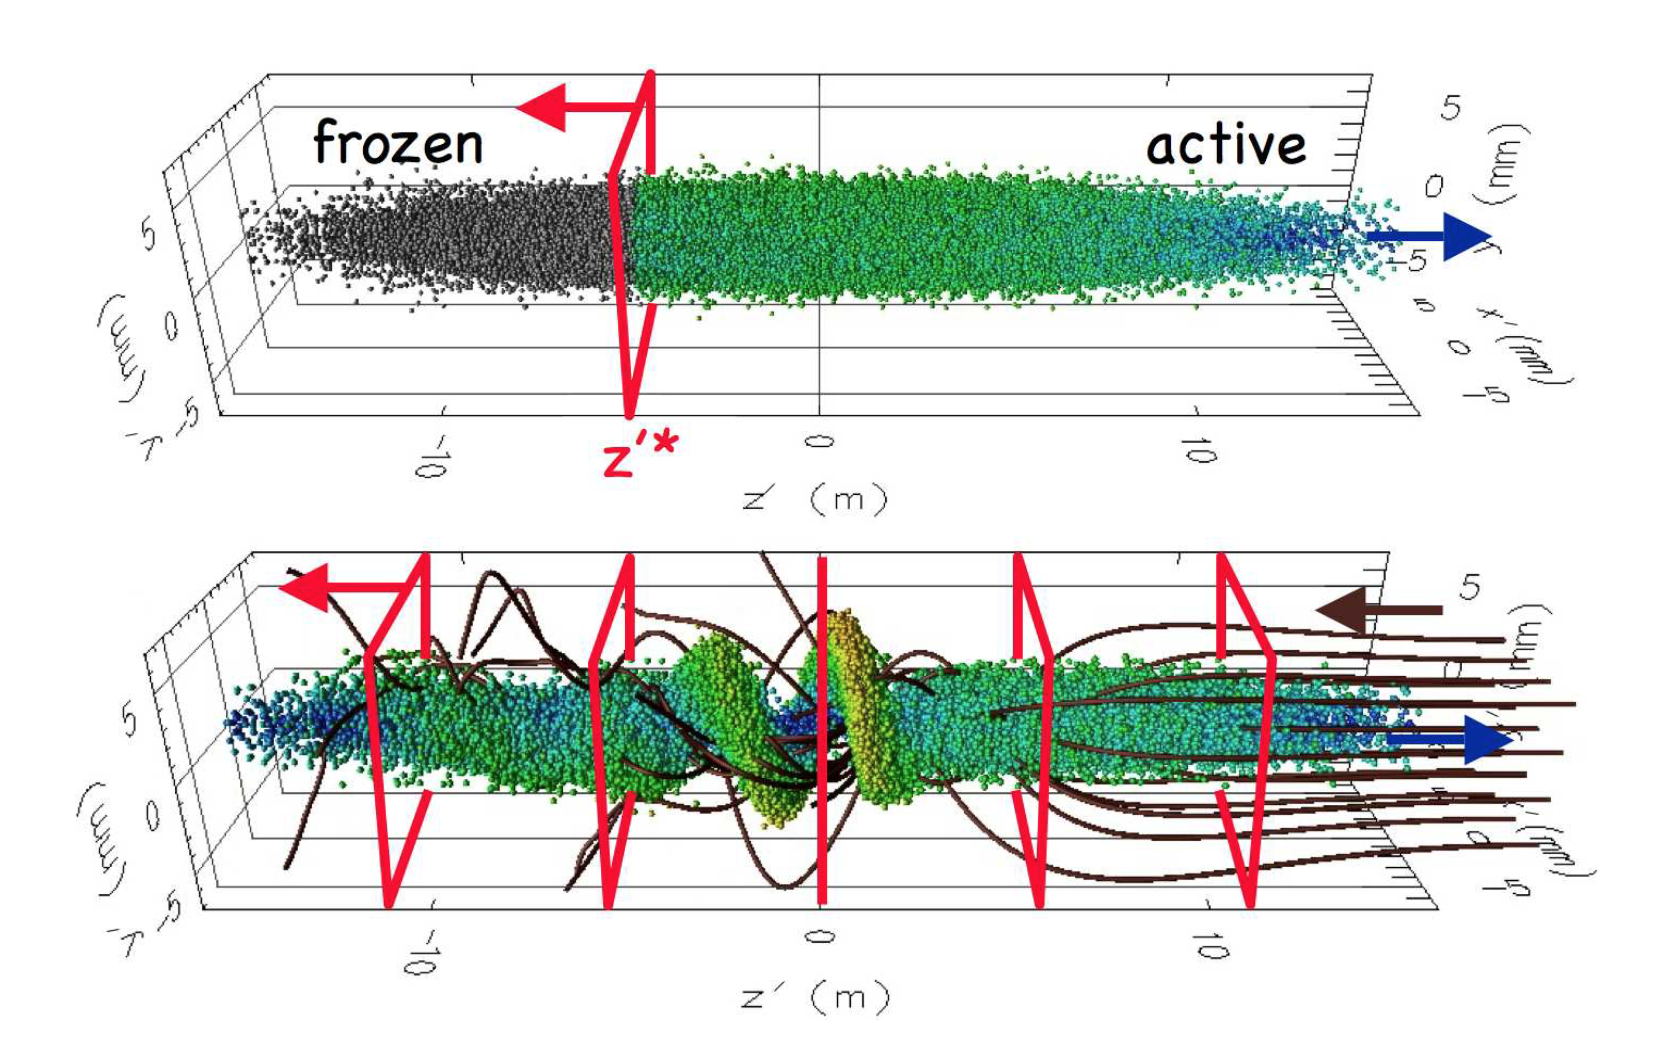
\includegraphics[width=120mm]{Input_output.png}
   \caption{(top) Snapshot of a particle beam showing ``frozen" (grey spheres) and ``active" (colored spheres) macroparticles traversing the injection plane (red rectangle). (bottom) Snapshot of the beam macroparticles (colored spheres) passing through the background of electrons (dark brown streamlines) and the diagnostic stations (red rectangles). The electrons, the injection plane and the diagnostic stations are fixed in the laboratory plane, and are thus counter-propagating to the beam in a boosted frame. }
   \label{Fig_inputoutput}
\end{figure}

The input and output data are often known from, or compared to, experimental data. Thus, calculating in
a frame other than the laboratory entails transformations of the data between the calculation frame and the laboratory
frame. This section describes the procedures that have been implemented in the Particle-In-Cell framework Warp \cite{Warp} to handle the input and output of data between the frame of calculation and the laboratory frame \cite{Vaypop2011}. Simultaneity of events between two frames is valid only for a plane that is perpendicular to the relative motion of the frame. As a result, the input/output processes involve the input of data (particles or fields) through a plane, as well as output through a series of planes, all of which are perpendicular to the direction of the relative velocity between the frame of calculation and the other frame of choice.

\subsubsection{Input in a boosted frame simulation}
\paragraph{Particles - }
Particles are launched through a plane using a technique that is generic and applies to Lorentz boosted frame simulations in general, including plasma acceleration, and is illustrated using the case of a positively charged particle beam propagating through a background of cold electrons in an assumed continuous transverse focusing system, leading to a well-known growing transverse ``electron cloud'' instability \cite{Vayprl07}. In the laboratory frame, the electron background is initially at rest and a moving window is used to follow the beam progression. Traditionally, the beam macroparticles are initialized all at once in the window, while background electron macroparticles are created continuously in front of the beam on a plane that is perpendicular to the beam velocity. In a frame moving at some fraction of the beam velocity in the laboratory frame, the beam initial conditions at a given time in the calculation frame are generally unknown and one must initialize the beam differently. However, it can be taken advantage of the fact that the beam initial conditions are often known for a given plane in the laboratory, either directly, or via simple calculation or projection from the conditions at a given time in the labortory frame. Given the position and velocity $\{x,y,z,v_x,v_y,v_z\}$ for each beam macroparticle at time $t=0$ for a beam moving at the average velocity $v_b=\beta_b c$ (where $c$ is the speed of light) in the laboratory, and using the standard synchronization ($z=z'=0$ at $t=t'=0$) between the laboratory and the calculation frames, the procedure for transforming the beam quantities for injection in a boosted frame moving at velocity $\beta c$ in the laboratory is as follows (the superscript $'$ relates to quantities known in the boosted frame while the superscript $^*$ relates to quantities that are know at a given longitudinal position $z^*$ but different times of arrival):

\begin{enumerate}
\item project positions at $z^*=0$ assuming ballistic propagation
\begin{eqnarray}
    t^* &=& \left(z-\bar{z}\right)/v_z \label{Eq:t*}\\
    x^* &=& x-v_x t^* \label{Eq:x*}\\
    y^* &=& y-v_y t^* \label{Eq:y*}\\
    z^* &=& 0 \label{Eq:z*}
\end{eqnarray}
the velocity components being left unchanged,
\item apply Lorentz transformation from laboratory frame to boosted frame
\begin{eqnarray}
    t'^* &=& -\gamma t^* \label{Eq:tp*}\\
    x'^* &=& x^* \label{Eq:xp*}\\
    y'^* &=& y^* \label{Eq:yp*}\\
    z'^* &=& \gamma\beta c t^* \label{Eq:zp*}\\
    v'^*_x&=&\frac{v_x^*}{\gamma\left(1-\beta \beta_b\right)} \label{Eq:vxp*}\\
    v'^*_y&=&\frac{v_y^*}{\gamma\left(1-\beta \beta_b\right)} \label{Eq:vyp*}\\
    v'^*_z&=&\frac{v_z^*-\beta c}{1-\beta \beta_b} \label{Eq:vzp*}
\end{eqnarray}
where $\gamma=1/\sqrt{1-\beta^2}$. With the knowledge of the time at which each beam macroparticle crosses the plane into consideration, one can inject each beam macroparticle in the simulation at the appropriate location and time.

\item synchronize macroparticles in boosted frame, obtaining their positions at a fixed $t'=0$ (before any particle is injected)
\begin{eqnarray}
    z' &=& z'^*-\bar{v}'^*_z t'^* \label{Eq:zp}
\end{eqnarray}
    This additional step is needed for setting the electrostatic or electromagnetic fields at the plane of injection. In a Particle-In-Cell code, the three-dimensional fields are calculated by solving the Maxwell equations (or static approximation like Poisson, Darwin or other \cite{Vaypop2008}) on a grid on which the source term is obtained from the macroparticles distribution. This requires generation of a three-dimensional representation of the beam distribution of macroparticles at a given time before they cross the injection plane at $z'^*$. This is accomplished by expanding the beam distribution longitudinally such that all macroparticles (so far known at different times of arrival at the injection plane) are synchronized to the same time in the boosted frame. To keep the beam shape constant, the particles are ``frozen'' until they cross that plane: the three velocity components and the two position components perpendicular to the boosted frame velocity are kept constant, while the remaining position component is advanced at the average beam velocity. As particles cross the plane of injection, they become regular ``active'' particles with full 6-D dynamics.

\end{enumerate}

Figure \ref{Fig_inputoutput} (top) shows a snapshot of a beam that has passed partly through the injection plane. As the frozen beam macroparticles pass through the injection plane (which moves opposite to the beam in the boosted frame), they are converted to ``active" macroparticles. The charge or current density is accumulated from the active and the frozen particles, thus ensuring that the fields at the plane of injection are consistent.

\paragraph{Laser - }

Similarly to the particle beam, the laser is injected through a plane perpendicular to the axis of propagation of the laser (by default $z$).
The electric field $E_\perp$ that is to be emitted is given by the formula
\begin{equation}
E_\perp\left(x,y,t\right)=E_0 f\left(x,y,t\right) \sin\left[\omega t+\phi\left(x,y,\omega\right)\right]
\end{equation}
where $E_0$ is the amplitude of the laser electric field, $f\left(x,y,t\right)$ is the laser envelope, $\omega$ is the laser frequency, $\phi\left(x,y,\omega\right)$ is a phase function to account for focusing, defocusing or injection at an angle, and $t$ is time. By default, the laser envelope is a three-dimensional gaussian of the form
\begin{equation}
 f\left(x,y,t\right)=e^{-\left(x^2/2 \sigma_x^2+y^2/2 \sigma_y^2+c^2t^2/2 \sigma_z^2\right)}
 \end{equation}
 where $\sigma_x$, $\sigma_y$ and $\sigma_z$ are the dimensions of the laser pulse; or it can be defined arbitrarily by the user at runtime.
If $\phi\left(x,y,\omega\right)=0$, the laser is injected at a waist and parallel to the axis $z$.

If, for convenience, the injection plane is moving at constant velocity $\beta_s c$, the formula is modified to take the Doppler effect on frequency and amplitude into account and becomes
\begin{eqnarray}
E_\perp\left(x,y,t\right)&=&\left(1-\beta_s\right)E_0 f\left(x,y,t\right)\nonumber \\
&\times& \sin\left[\left(1-\beta_s\right)\omega t+\phi\left(x,y,\omega\right)\right].
\end{eqnarray}

The injection of a laser of frequency $\omega$ is considered for a simulation using a boosted frame moving at $\beta c$ with respect to the laboratory. Assuming that the laser is injected at a plane that is fixed in the laboratory, and thus moving at $\beta_s=-\beta$ in the boosted frame, the injection in the boosted frame is given by
\begin{eqnarray}
E_\perp\left(x',y',t'\right)&=&\left(1-\beta_s\right)E'_0 f\left(x',y',t'\right)\nonumber \\
&\times&\sin\left[\left(1-\beta_s\right)\omega' t'+\phi\left(x',y',\omega'\right)\right]\\
&=&\left(E_0/\gamma\right) f\left(x',y',t'\right) \nonumber\\
&\times&\sin\left[\omega t'/\gamma+\phi\left(x',y',\omega'\right)\right]
\end{eqnarray}
since $E'_0/E_0=\omega'/\omega=1/\left(1+\beta\right)\gamma$.

The electric field is then converted into currents that get injected via a 2D array of macro-particles, with one positive and one dual negative macro-particle for each array cell in the plane of injection, whose weights and motion are governed by $E_\perp\left(x',y',t'\right)$. Injecting using this dual array of macroparticles offers the advantage of automatically including the longitudinal component that arises from emitting into a boosted frame, and to automatically verify the discrete Gauss' law thanks to using charge conserving (e.g. Esirkepov) current deposition scheme \cite{Esirkepovcpc01}.

\subsubsection{Output in a boosted frame simulation}
Some quantities, e.g. charge or dimensions perpendicular to the boost velocity, are Lorentz invariant.
Those quantities are thus readily available from standard diagnostics in the boosted frame calculations. Quantities that do not fall in this category are recorded at a number of regularly spaced ``stations", immobile in the laboratory frame, at a succession of time intervals to record data history, or averaged over time. A visual example is given on Fig.  \ref{Fig_inputoutput} (bottom). Since the space-time locations of the diagnostic grids in the laboratory frame generally do not coincide with the space-time positions of the macroparticles and grid nodes used for the calculation in a boosted frame, some interpolation is performed at runtime during the data collection process. As a complement or an alternative, selected particle or field quantities can be dumped at regular intervals and quantities are reconstructed in the laboratory frame during a post-processing phase. The choice of the methods depends on the requirements of the diagnostics and particular implementations.
